\iffalse
\chapter{2024}
\author{AI24BTECH11022}
\section{ae}
\fi

\usetikzlibrary{patterns}
\item In the figure shown below, the magnitude of internal force in member $BC$
is \rule{1cm}{0.15mm} $N$ (rounded off to $1$ decimal place).\hfill(2024)

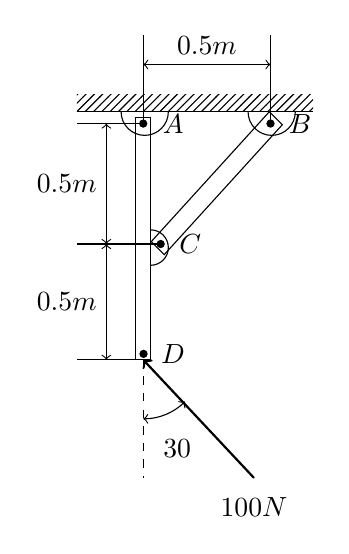
\begin{tikzpicture}[scale=1.5]
\draw (0,0) rectangle (0.125,2.05);
\draw[thick,->] (1,-1) -- (0.0625,0);
\node at (1,-1.25) {$100N$};
\draw[dashed] (0.0625,0) -- (0.0625,-1);
\draw[<->] (0.0625,-0.5) arc (-90:-45:0.5);
\node at (0.35,-0.75) {$30\degree$};
\fill[pattern=north east lines] (-0.5,2.1) rectangle (1.5,2.25);
\draw (-0.125,2.1) arc (180:360:0.2);
\fill (0.0625,2) circle (1pt);
\draw (0.125,0.8) arc (-90:90:0.15);
\draw (0.13,1) -- (1.13,2.1) -- (1.24,1.99) -- (0.24,0.89) -- (0.13,1);
\fill (0.21,0.98) circle (1pt);
\draw (-0.5,2.1) -- (1.5,2.1);
\draw (0.95,2.1) arc (180:360:0.2);
\fill (1.14,2) circle (1pt);
\draw (0.0625,2) -- (0.0625,2.75);
\draw (1.14,2) -- (1.14,2.75);
\draw (0.0625,2) -- (-0.5,2);
\draw (0.21,0.98) -- (-0.5,0.98);
\draw (0,0) -- (-0.5,0);
\draw[<->] (-0.25,0) -- (-0.25,0.98) node[midway,left] {$0.5m$};
\draw[<->] (-0.25,0.98) -- (-0.25,2) node[midway,left] {$0.5m$};
\draw[<->] (0.0625,2.5) -- (1.14,2.5) node[midway,above] {$0.5m$};
\node at (0.31625,2) {$A$};
\node at (0.46,0.98) {$C$};
\node at (1.39,2) {$B$};
\fill (0.065,0.05) circle (1pt);
\node at (0.315,0.05) {$D$};
\end{tikzpicture}


\item The cross section of a thin-walled beam with uniform wall thickness $t$, shown in the figure, is subjected to a bending moment $M_{x}=10Nm$. If $h=1m$ and $t=0.001m$, the magnitude of maximum normal stress in the cross section is \rule{1cm}{0.15mm} $N/m^{2}$ (answer in integer).\hfill(2024)

\begin{tikzpicture}[scale=1.25]
\draw (0,0) -- (2,0) -- (2,-0.5);
\draw (3,0) -- (3,-0.5);
\draw[->] (1,1) -- (5,1) node[right] {$x$};
\draw (0,2) -- (2,2);
\draw (3,2) -- (3,2.5);
\draw[->] (2,2) -- (2,3) node[above] {$y$};
\draw[<->] (0.75,0) -- (0.75,2) node[midway,left] {$h$};
\draw[->] (1.25,-0.25) -- (2,-0.25);
\draw[->] (1.25,2.25) -- (2,2.25);
\draw[->] (3.75,-0.25) -- (3,-0.25);
\draw[->] (3.75,2.25) -- (3,2.25);
\draw[ultra thick] (3,0) -- (2,0) node[midway,below] {$\frac{h}{2}$} -- (2,2) -- (3,2) node[midway,above] {$\frac{h}{2}$};
\draw[->] (1.25,1.75) -- (2,1.75);
\draw[->] (2.75,1.75) -- (2,1.75);
\node at (2.9,1.75) {$t$};
\end{tikzpicture}

\item The equations of motion for a two degrees of freedom undamped spring-mass system are : $$mx_{1}+2kx_{1}-kx_{2}=0$$ $$mx_{2}-kx_{1}+2kx_{2}=0$$ where $m$ and $k$ represent mass and stiffness respectively, in corresponding SI units, and $x_{1}$ and $x_{2}$ are the degrees of freedom. The larger of the two natural frequencies is given by: $\omega=\alpha\sqrt{\frac{k}{m}}rad/s$. The value of $\alpha$ is \rule{1cm}{0.15mm} (rounded off to 2 decimal places).\hfill(2024)


\item Consider the plane strain field given by $$\epsilon_{xx}=10xy^{2},\epsilon_{yy}=-5x^{2}y\text{ and }\gamma_{xy}=Axy\brak{2x-y}$$ where, $A$ is a constant and $\gamma_{xy}$ is the engineering shear strain. The value of the constant $A$ for the strain field to be compatible is \rule{1cm}{0.15mm} (rounded off to $1$ decimal place).\hfill(2024)


\item A chemical rocket with an ideally expanded flow through the nozzle produces $5\times 10^{6}N$ thrust at sea level. The specific impulse of the rocket is $200s$ and acceleration due to gravity at the sea level is $9.8m/s^{2}$. The propellent mass flow rate out of the rocket nozzle is \rule{1cm}{0.15mm} $kg/s$ (rounded off to the nearest integer).\hfill(2024)


\item A centrifugal compressor is designed to operate with air. At the leading edge of the tip of the inducer (eye of the impeller), the blade angle is $45\degree$, and the relative Mach number is $1.0$. The stagnation temperature of the incoming air is $300K$. Consider $\gamma=1.4$. Neglect pre-whirl and slip. The inducer tip speed is \rule{1cm}{0.15mm} $m/s$ (rounded off to the nearest integer).\hfill(2024)


\item Consider the following Fanno flow problem: Flow enters a constant area duct at a temperature of $273K$ and a Mach number $0.2$ and eventually reaches sonic condition (Mach number $=1$) due to friction. Assume $\gamma=1.4$. The static temperature at the location where sonic condition is reached is \rule{1cm}{0.15mm} $K$ (rounded off to $2$ decimal places).\hfill(2024)


\item Consider an artificial satellite moving around the Moon in an elliptic orbit. The altitude of the satellite from the Moon's surface at the perigee is $25km$ and that at the apogee is $134km$. Assume the Moon to be spherical with a radius of $1737km$. The trajectory is considered with reference to a coordinate system fixed to the center of mass of the Moon. The ratio of the speed of the satellite at the perigee to that at the apogee is \rule{1cm}{0.15mm} (rounded off to $2$ decimal places).\hfill(2024)


\item For an aircraft moving at $4km$ altitude above mean sea level at a Mach number of $0.2$, the ratio of equivalent air speed to true air speed is \rule{1cm}{0.15mm} (rounded off to $2$ decimal places).\\

The density of air at mean sea level is $1.225kg/m^{3}$ and at $4km$ altitude is $0.819kg/m^{3}$.\hfill(2024)


\item For a general aviation airplane, one of the complex conjugate pair of eigenvalues for longitudinal dynamics is given by $-0.039\pm 0.0567i$ (in SI units). If the system is disturbed to excite only this mode, the time taken for the amplitude of response to become half in magnitude is \rule{1cm}{0.15mm} $s$ (rounded off to $1$ decimal place).\hfill(2024)


\item The figure (not to scale) shows a control volume to estimate the forces on the airfoil with elliptic cross-section. Surfaces $2$ and $3$ are streamlines. Velocity profiles are measured at the upstream end (surface $1$) and at the downstream end (surface $4$) of the control volume. The drag coefficient for the airfoil is defined as $C_{d}=\frac{D}{\frac{1}{2}\rho U_{\infty}^{2}c}$, where $D$ is the drag force on the airfoil per unit span and $\rho$ is the density of the air. The static pressure, $p_{\infty}$, is constant over the entire surface of the control volume. Assuming the flow to be incompressible, two-dimensional and steady, the $C_{d}$ for the airfoil is \rule{1cm}{0.15mm} (rounded off to $3$ decimal places).\hfill(2024)

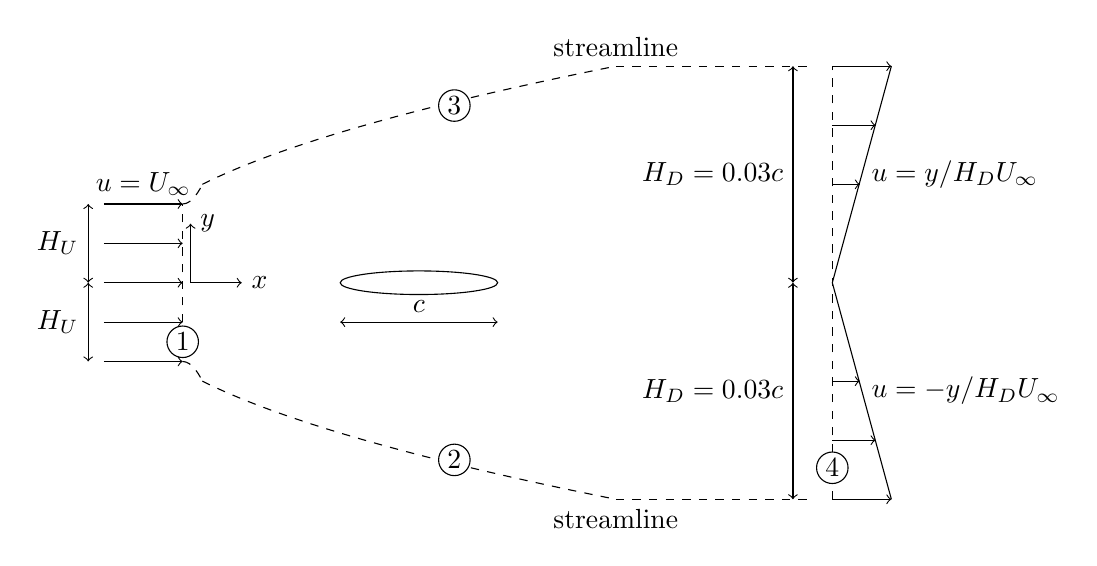
\begin{tikzpicture}
\foreach \x in {-2,-1,0,1,2} {
\draw[->] (0,\x/2) -- (1,\x/2);
}
\draw[<->] (-0.2,-1) -- (-0.2,0) node[midway,left] {$H_{U}$};
\draw[<->] (-0.2,1) -- (-0.2,0) node[midway,left] {$H_{U}$};
\node at (0.5,1.25) {$u=U_{\infty}$};
\draw[dashed] (1,-0.5) -- (1,1);
\draw (1,-0.75) circle (0.2cm);
\node at (1,-0.75) {$1$};
\draw[->] (1.1,0) -- (1.75,0) node[right] {$x$};
\draw[->] (1.1,0) -- (1.1,0.75) node[right] {$y$};
\draw[dashed] (1,1) parabola (1.25,1.25);
\draw[dashed] (1,-1) parabola (1.25,-1.25);
\draw[dashed] plot[smooth,domain=1:2] ({\x^2+0.25},\x+0.25);
\draw[dashed] plot[smooth,domain=1:2] ({\x^2+0.25},-\x-0.25);
\draw (4.45,2.25) circle (0.2cm);
\node at (4.45,2.25) {$3$};
\draw (4.45,-2.25) circle (0.2cm);
\node at (4.45,-2.25) {$2$};
\draw[dashed] plot[smooth,domain=2.1:2.5] ({\x^2+0.25},\x+0.25);
\draw[dashed] plot[smooth,domain=2.1:2.5] ({\x^2+0.25},-\x-0.25);
\draw[dashed] (6.5,2.75) -- (9,2.75);
\draw[dashed] (6.5,-2.75) -- (9,-2.75);
\draw[<->] (8.75,0) -- (8.75,2.75) node[midway,left] {$H_{D}=0.03c$};
\draw[<->] (8.75,0) -- (8.75,-2.75) node[midway,left] {$H_{D}=0.03c$};
\draw[dashed] (9.25,-2.15) -- (9.25,2.75);
\draw[dashed] (9.25,-2.75) -- (9.25,-2.55);
\draw (9.25,-2.35) circle (0.2cm);
\node at (9.25,-2.35) {$4$};
\draw (10,2.75) -- (9.25,0) node[midway,right] {$u=\brak{y/H_{D}}U_{\infty}$} -- (10,-2.75) node[midway,right] {$u=\brak{-y/H_{D}}U_{\infty}$};
\draw[->] (9.25,-2.75) -- (10,-2.75);
\draw[->] (9.25,-2) -- (9.8,-2);
\draw[->] (9.25,-1.25) -- (9.6,-1.25);
\draw[->] (9.25,2.75) -- (10,2.75);
\draw[->] (9.25,2) -- (9.8,2);
\draw[->] (9.25,1.25) -- (9.6,1.25);
\node at (6.5,3) {streamline};
\node at (6.5,-3) {streamline};
\draw[<->] (3,-0.5) -- (5,-0.5) node[midway,above] {$c$};
\draw (4,0) ellipse (1cm and 0.15cm);
\end{tikzpicture}


\item An airplane of mass $1000kg$ is in a steady level flight with a speed of $50m/s$. The wing has an elliptic planform with a span of $20m$ and planform area $31.4m^{2}$. Assuming the density of air at that altitude to be $1kg/m^{3}$ and acceleration due to gravity to be $10m/s^{2}$, the induced drag on the wing is \rule{1cm}{0.15mm} $N$ (rounded off to $1$ decimal place).\hfill(2024)


\item It is desired to estimate the aerodynamic drag, $D$, on a car traveling at a speed of $30m/s$. A one-third scale model of the car is tested in a wind-tunnel following the principles of dynamic similarity. The drag on the scaled model is measured to be $D_{m}$. The ratio $D/D_{m}$ is \rule{1cm}{0.15mm} (rounded off to $1$ decimal place).\hfill(2024)